\section{Standard Containers}
There are three main types of standard containers in the C++ language. \\ Containers can be: default-constructed, copy-constructed from another container of the same type, equality compared, emptied with clear().
\begin{itemize}
	\itemsep -0.5em
	\item Sequence Containers
		\SubItem{Elements are accessible in order as they were inserted/created.}
		\SubItem{Find in linear time through the algorithm find.}
	\item Associative Containers
		\SubItem{Elements are accessible in sorted order}
		\SubItem{find as member function in logarithmic time}
	\item Hashed Containers
		\SubItem{Elements are accessible in unspecified order}
		\SubItem{find as member function in constant time}
\end{itemize}

\begin{figure}[h!]
  \centering
  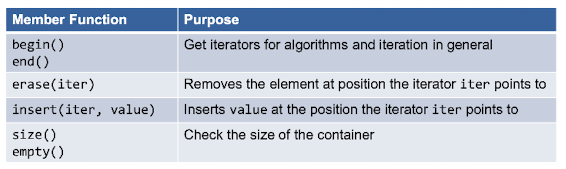
\includegraphics[width=0.75\linewidth]{container}
  \caption{Member Function of a Container}
\end{figure}

\subsection{Common Container Constructors}

\begin{lstlisting}[language=C++]
// Constructor with Initializer List
std::vector<int> v{1,2,3,5,6,11};
// Construction with a number of elements, five times a 42
std::list<int> l(5,42);
// Range with a pair of iterators
std::deque<int> q{begin(v), end(v)};
\end{lstlisting}

\subsection{Sequence Container}
std::vector<T>, std::deque<T>, std::list<T>, std::array<N, T>.\\
Defines order of elements as inserted/appended to the container. Lists are very good for splicing and in the middle insertions. Array and deque are very efficient unless bad usage.

\begin{figure}[h!]
 	\centering
 	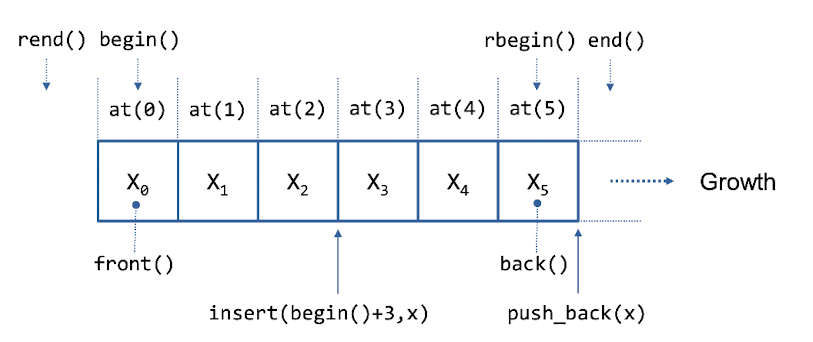
\includegraphics[width=0.6\linewidth]{sequencecontainer}
  \caption{}
\end{figure}

% TODO add all containers

\subsection{Associated Containers}
Can be searched by content and not by sequence. 

\begin{figure}[h!]
  \centering
  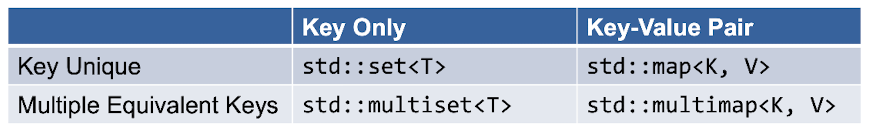
\includegraphics[width=0.6\linewidth]{associativecontainer}
  \caption{}
\end{figure}

%TODO add data types

\subsection{Hashed Containers}
Introduced in C++11. Standard lacks feature for creating your own hash functions. 

\subsection{Iterators}
Different containers support iterators of different capabilities. Categories are formed around increasing "power".

\textbf{Input Iterator} \\
Supports reading the "current" element (of type Element). Allows for one-pass input algorithms.  Can be compared with == and !=. Can also be copied.

\begin{lstlisting}[language=C++]
struct input_iterator_tag{};

Element operator*();
It & operator++(); 
It operator++(int); 
bool operator==(It const &); 
bool operator!=(It const &); 
It & operator=(It const &); 
It(It const &); //copy ctor
\end{lstlisting}

\textbf{Forward Iterator} \\
Can do whatever an input iterator can do plus: supports changing the current element. Still allows only for one-pass input algorithms.
\begin{lstlisting}[language=C++]
struct forward_iterator_tag{};
Element & operator*(); 
It & operator++(); 
It operator++(int); 
bool operator==(It const &); 
bool operator!=(It const &); 
It & operator=(It const &); 
It(It const &); //copy ctor
\end{lstlisting} 

\textbf{Bidirectional Iterator}\\
Can do whatever the forward iterator can do plus going backwards.
\begin{lstlisting}[language=C++]
struct bidirectional_iterator_tag{};
It & operator--(); 
It operator--(int); 
\end{lstlisting}

\textbf{Random Access Iterator} \\
Can do what the bidiretional iterator can do plus: Directly access element at index (offset to current position): distance can be positive or negative, Go n steps forward or backward, "Subtact" two iterators to get the distance, Compare with relational operators (<, <=, >, >=).
 Allows also random access in algorithms.

\textbf{Output Iterators} \\
 Can write value to current element, but only once (\*it = value).  Modeled after std::ostream\_iterator. 

\begin{lstlisting}[language=C++]
struct output_iterator_tag{};
Element & operator*(); 
It & operator++(); 
It operator++(int);
\end{lstlisting}

\subsubsection{Iterator Functions}
Has two functions std::distance(start, goal); std::advance(itr, n);.

\begin{lstlisting}[language=C++]
int main() {
std::vector<int> primes{2, 3, 5, 7, 11, 13};
auto current = std::begin(primes); auto afterNext = std::next(current); std::cout << "current: " << *current << " afterNext: " << *afterNext << '\n';
std::advance(current, 1); std::cout << "current: " << *current << " afterNext: " << *afterNext << '\n';
}
\end{lstlisting}


\pagebreak
